According to the operation principle, WPT systems can be categorized as \textit{maximum power transfer} that maximizes the coverage and \textit{maximum energy efficiency transfer} \cite{Hui2014} that compromise with the power budget. Figure \ref{fig:wpt-block-diagram} illustrates the fundamental blocks of a generic WPT system.

\begin{figure}\label{fig:wpt-block-diagram}
  \caption{Block diagram of a conventional far-field WPT architecture \cite{Clerckx2018a}}
  \centering
    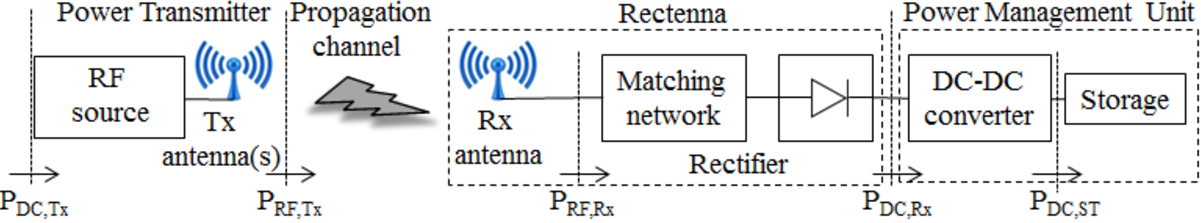
\includegraphics[width=0.5\textwidth]{Block diagram of a conventional far-field WPT architecture}
\end{figure}

The transmit power efficiency $e$ is decomposed as:

\begin{equation}\label{eqn:power_utilization_efficiency}
  e = \frac{{{P_{{\text{dc}},{\text{ST}}}}}}{{P_{{\text{dc}}}^t}} = \underbrace {\frac{{P_{{\text{rf}}}^t}}{{P_{{\text{dc}}}^t}}}_{{e_1}} \cdot \underbrace {\frac{{P_{{\text{rf}}}^r}}{{P_{{\text{rf}}}^t}}}_{{e_2}} \cdot \underbrace {\frac{{P_{{\text{dc}}}^r}}{{P_{{\text{rf}}}^r}}}_{{e_3}} \cdot \underbrace {\frac{{{P_{{\text{dc}},{\text{ST}}}}}}{{P_{{\text{dc}}}^r}}}_{{e_4}}
\end{equation}

Most existing solutions assumed no dependency for the components and focused on maximizing each term individually. Nevertheless, it has been proved by \cite{Boshkovska2015, Clerckx2016, Zeng2017} that these efficiencies are indeed coupled with each other, especially when input power is low (below 1~mW). Specifically, the DC-to-RF efficiency ${e_1}$ is related to the Peak-to-Average Power Ratio (PAPR) hence the waveform \cite{Boaventura2011}. Similarly, the RF-to-RF efficiency ${e_2}$ is determined by the channel state and the signal characteristics as waveform, beamformer, modulation, and power allocation \cite{Clerckx2019}. It also desires a highly directional transmission \cite{Takahashi2011}. ${e_3}$ measures the RF-to-DC efficiency of the rectenna, which is sensitive to the diode characteristics, parasitic sources, impedance matching, and harmonic generation \cite{Strassner2013, Valenta2014}. It is also related to the rectifier input power ${P_{{\text{rf}}}^r}$ \cite{Trotter2009, Chen2017, Clerckx2018a}, channel and the transmit signal \cite{Collado2014, Boaventura2015, Clerckx2019}. The DC-to-DC efficiency ${e_4}$ can be maximized by dynamically adjusting the rectifier load with the diode impedance \cite{Dolgov2010}. From the perspective of WPT, this article particularly investigates the relationship between waveform design and ${e_2} \cdot {e_3}$ based on the nonlinear harvester model proposed in \cite{Clerckx2016}. 
